\documentclass{article}
% translate with >> pdflatex -shell-escape <file>

% This file is an extract of the PGFPLOTS manual, copyright by Christian Feuersaenger.
% 
% Feel free to use it as long as you cite the pgfplots manual properly.
%
% See
%   http://pgfplots.sourceforge.net/pgfplots.pdf
% for the complete manual.
%
% Any required input files (for <plot table> or <plot file> or the table package) can be downloaded
% at
% http://www.ctan.org/tex-archive/graphics/pgf/contrib/pgfplots/doc/latex/
% and
% http://www.ctan.org/tex-archive/graphics/pgf/contrib/pgfplots/doc/latex/plotdata/

\usepackage{pgfplots}
\pgfplotsset{compat=newest}

\pagestyle{empty}
\usetikzlibrary{decorations.markings}

\begin{document}
% requires \usetikzlibrary{decorations.markings}
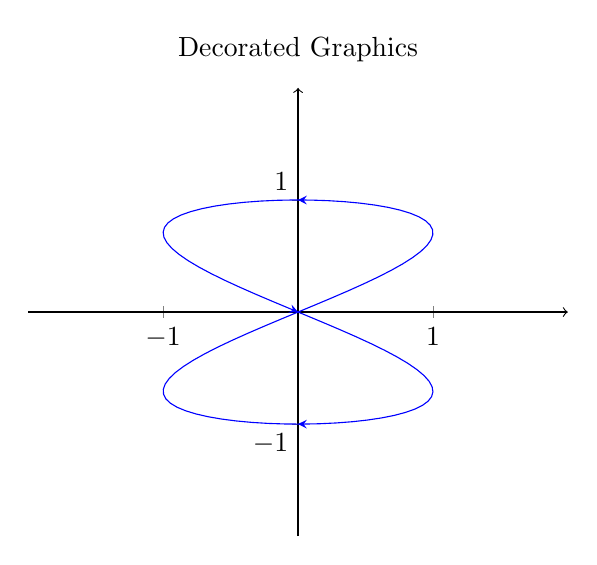
\begin{tikzpicture}[]
% Same as in previous example, but with decorations:
\begin{axis}[axis lines=middle,
	title=Decorated Graphics,
	xmin=-2, xmax=2, ymin=-2, ymax=2,
	xtick={-1,1}, ytick={-1,1},
	% this disables the standard 
	% tick label *text* (but not the line)
	yticklabel=\ ,
	extra description/.code={
		% this generates custom y labels to implement 
		% individual styles for every tick:
		\node[below left] at (axis cs:0,-1) {$-1$};
		\node[above left] at (axis cs:0,1) {$1$};
	},
	axis line style={->},
  ]
  \addplot[blue,samples=100,domain=0:2*pi,
	postaction={decorate},% ------
	decoration={markings, % ------
		 mark=at position 0.25 with {\arrow{stealth}},
		 mark=at position 0.5  with {\arrow{stealth}},
		 mark=at position 0.75 with {\arrow{stealth}}}
	]
	({sin(deg(2*x))}, {sin(deg(x))});
\end{axis}
\end{tikzpicture}
\end{document}
